\documentclass[12pt, titlepage]{article}

\usepackage{booktabs}
\usepackage{tabularx}
\usepackage{hyperref}
\usepackage{graphicx}
\usepackage{amsmath, mathtools}
\usepackage{amsfonts}
\usepackage{amssymb}
\usepackage{graphicx}
\usepackage{colortbl}
\usepackage{xr}
\usepackage{hyperref}
\usepackage{longtable}
\usepackage{xfrac}
\usepackage{tabularx}
\usepackage{float}
\usepackage{siunitx}
\usepackage{booktabs}
\usepackage{caption}
\usepackage{pdflscape}
\usepackage{afterpage}
\hypersetup{
    colorlinks,
    citecolor=black,
    filecolor=black,
    linkcolor=red,
    urlcolor=blue
}
\usepackage[round]{natbib}

\newcounter{tnum}
\newcommand{\tthetestnum}{\thetnum}
\newcommand{\tref}[1]{T\ref{#1}}

%% Comments

\usepackage{color}

\newif\ifcomments\commentstrue

\ifcomments
\newcommand{\authornote}[3]{\textcolor{#1}{[#3 ---#2]}}
\newcommand{\todo}[1]{\textcolor{red}{[TODO: #1]}}
\else
\newcommand{\authornote}[3]{}
\newcommand{\todo}[1]{}
\fi

\newcommand{\wss}[1]{\authornote{blue}{SS}{#1}}
\newcommand{\an}[1]{\authornote{magenta}{Author}{#1}}
\newcommand{\wss}[1]{\authornote{blue}{SS}{#1}}



\begin{document}

\title{FFT Library} 
\author{Yuzhi Zhao}
\date{\today}
	
\maketitle

\pagenumbering{roman}

\section{Revision History}

\begin{tabularx}{\textwidth}{p{3cm}p{2cm}X}
\toprule {\bf Date} & {\bf Version} & {\bf Notes}\\
\midrule
Date 1 & 1.0 & Notes\\
Date 2 & 1.1 & Notes\\
\bottomrule
\end{tabularx}

~\newpage

\section{Symbols, Abbreviations and Acronyms}

\renewcommand{\arraystretch}{1.2}
\begin{tabular}{l l} 
  \toprule		
  \textbf{symbol} & \textbf{description}\\
  \midrule 
  T & Test\\
  FFT & Fast Fourier Transform\\
IFFT & Inverse Fast Fourier Transform\\
CA & Commonality Analysis\\
IM & Instance Module\\
MSE & Mean Squared Error\\
$o_i $ & Output Data\\
$e_i$ & Expected Output Data\\
  \bottomrule
\end{tabular}\\

\newpage

\tableofcontents

\listoftables

\listoffigures

\newpage

\pagenumbering{arabic}


\section{General Information}
The following section provides an overview of the Verification and Validation (V \& V) Plan for a FFT library.

\subsection{Purpose}
The main purpose of this document is to describe the verification and validation process
that will be used to test a FFT Library.This document is intended to be used as a reference for all future testing and will be used
to increase confidence in the software implementation.\\
This document will be used as a starting point for the verification and validation report.
The test cases presented within this document will be executed and the output will be
analyzed to determine if the library is implemented correctly.

\subsection{Scope}
The whole library includes four FFT or IFFT calculation functions. All tests should be applied based on this scope.

\subsection{Overview of Document}
The following sections provides more details about the V\&V of a FFT Library. Information about verification tools, automated testing approaches will be stated. And
test cases for all system testing and part of unit testing will be provided.
\section{Plan}
	
\subsection{Software Description}
The software being tested is a library for FFT algorithm. Users choose different  FFT or IFFT functions and give proper input datas to complete a FFT or IFFT calculation. 
The library includes radix-2 and radix-3 FFT(and IFFT) calculation functions.
\subsection{Test Team}
Yuzhi Zhao

\subsection{Automated Testing Approach}
A unit testing framework will be implemented in both unit testing and system testing.\\
Script will be used to call all the test cases in test suite.\\
Test coverage analysis will be applied to measure code coverage.\\
Compiler can do syntax check automatically.

\subsection{Verification Tools}
\begin{enumerate}
\item {{\large Cutest} as unit testing framework}
\item {{\large Make} as script to call test cases and execute test}
\item {{\large Xcover} as coverage analysis tool}
\end{enumerate}

% \subsection{Testing Schedule}
		
% See Gantt Chart at the following url ...

\subsection{Non-Testing Based Verification}
{\large Symbolic Execution}

Because FFT library is based on a mathematical expression. Using Symbolic Execution can trace the path and the result can be compared with mathematical expression directly.



\section{System Test Description}
	
\subsection{Tests for Functional Requirements}

\subsubsection{Calculation Test}
		
\paragraph{Radix-2 Complex Number Calculation Function\\}

\begin{enumerate}

\item{\textbf{T-\refstepcounter{tnum}\thetnum \label{R2CFFT}:Radix-2 Complex Number FFT Calculation Function}}

\textbf {Type}: Functional, Dynamic, Automated
					
\textbf {Initial State}: None
					
\textbf {Input}:\\{\large input.txt} :  Includes all the input datas. Two examples of input.txt is shown in Figure~\ref{Fig_Inputcomplex} and Figure~\ref{Fig_Inputfloating}. The floating numbers can be generated by random number generator online. The source can be reached using    \url  {http://www.meridianoutpost.com/resources/etools/calculators/generator-random-real.php?} The integer numbers can be generated using \url {https://andrew.hedges.name/experiments/random/}.\\\\ 
{\large expectedOutput.txt}:  Includes the output datas using the same input datas but computed by Matlab FFT library. Then expectedOutput.txts  are shown in Figure~\ref{Fig_OutputComplex} and Figure~\ref{Fig_Outputfloating}. \\ 
If the numbers of data can not satisfy $2^n$, program will automatically fill with 0.\\
					
\textbf {Output}: \\{\large output.txt} : Includes the output datas using the input data computed by this FFT library.\\
{\large TestResult}: pass or not pass. Whether the program passed the test is measured by an admissible error and the Mean Squared Error will be used as the algorithm. The equation is provided below:\\\\
\begin{gather}
MSE = \frac{1}{n}\sum_{i=0}^{n-1} (o_i - e_i)^2
\end{gather}
$e$ means expected output. $o$ means this library's output.\\
If the value of MSE is below 1\% of average of input datas, then this library passed the test.


			
\textbf {How test will be performed}: \\
Automated.\\
For validation purpose, datas should also be compared with results from normal DFT calculations as well. Do the same test as above but fill the output.txt with results from using DFT library.

\item{\textbf{T-\refstepcounter{tnum}\thetnum \label{R2CFFT}:Radix-2 Complex Number IFFT Calculation Function}}

\textbf {Type}: Functional, Dynamic, Automated
					
\textbf {Initial State}: None
					
\textbf {Input}:\\{\large input.txt} :  Includes all the input datas. The datas of  input testing file can use the same datas from output.txt from T- 1 shown in Figure~\ref{Fig_OutputComplex} and Figure~\ref{Fig_Outputfloating}. \\ \\
{\large expectedOutput.txt}:  Includes the output datas using the same input datas but computed by Matlab IFFT library.\\ 
If the numbers of data can not satisfy $2^n$, program will automatically fill with 0.\\
					
\textbf {Output}: \\{\large output.txt} : Includes the output datas using the input data computed by this IFFT library.\\
{\large TestResult}: pass or not pass. Whether the program passed the test is measured by an admissible error and the algorithm is same as it in T-1.\\
\textbf {How test will be performed}: \\
Same as above.
\end{enumerate}


\begin{figure}[h!]
\centering
\begin{minipage}[b]{0.38\textwidth}
 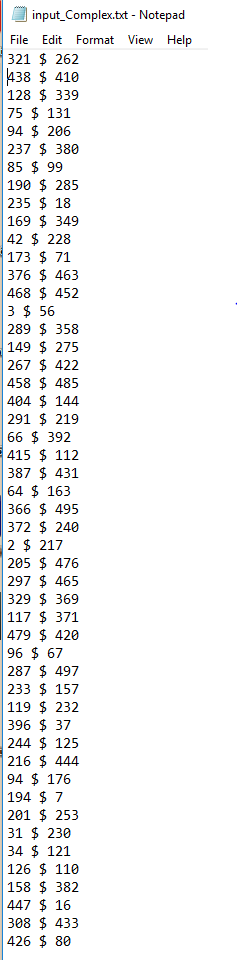
\includegraphics[width=\textwidth]{Input_complex}
\caption{Complex Integer Numbers As Input}
\label{Fig_Inputcomplex} 
\end{minipage}
\hfill
\begin{minipage}[b]{0.31\textwidth}
 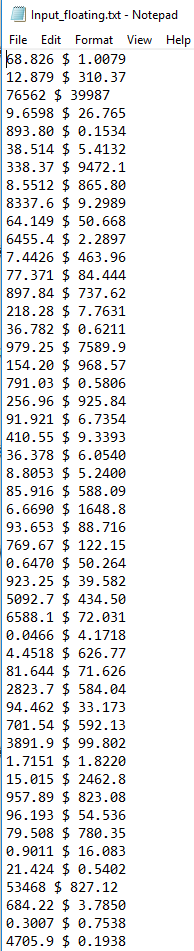
\includegraphics[width=\textwidth]{Input_floating}
\caption{Complex Floating Numbers As Input}
\label{Fig_Inputfloating} 
\end{minipage}
\end{figure}

\begin{figure}[h!]
\centering
\begin{minipage}[b]{0.44\textwidth}
 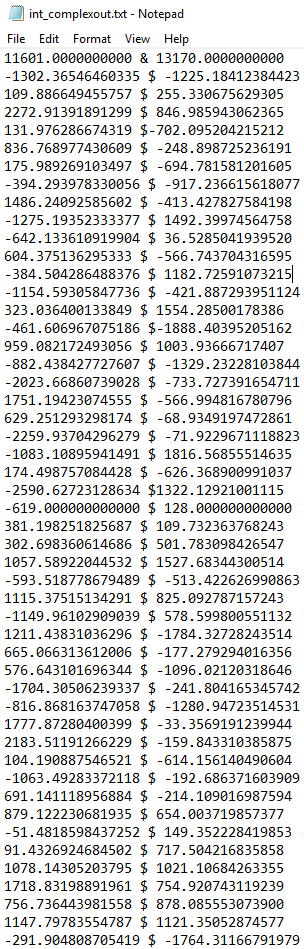
\includegraphics[width=\textwidth]{Output_Complex}
\caption{Output For Integer Complex Numbers As Input}
\label{Fig_OutputComplex} 
\end{minipage}
\hfill
\begin{minipage}[b]{0.49\textwidth}
 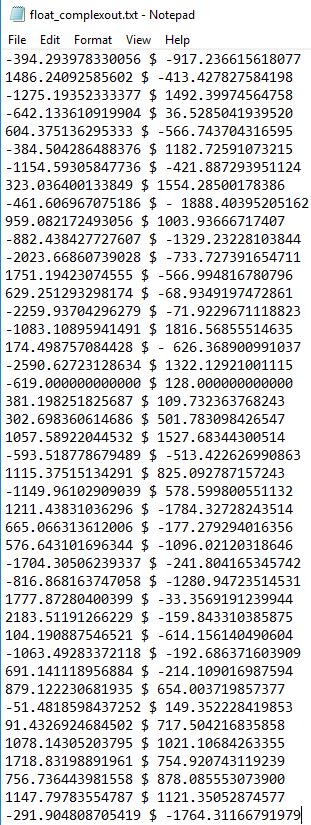
\includegraphics[width=\textwidth]{Output_floatingComplex}
\caption{Output For Floating Complex Numbers As Input}
\label{Fig_Outputfloating} 
\end{minipage}
\end{figure}
		
\begin{figure}[h!]
\centering
\begin{minipage}[b]{0.32\textwidth}
 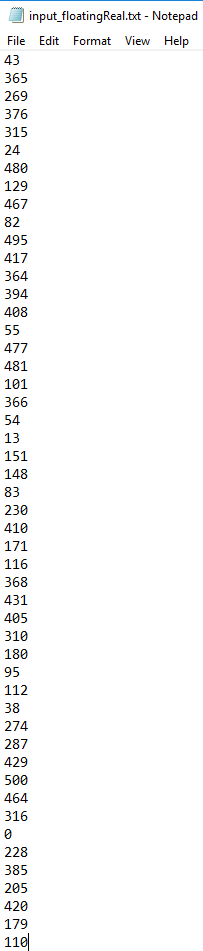
\includegraphics[width=\textwidth]{Input_real}
\caption{Real Integer Numbers As Input}
\label{Fig_Inputreal} 
\end{minipage}
\hfill
\begin{minipage}[b]{0.31\textwidth}
 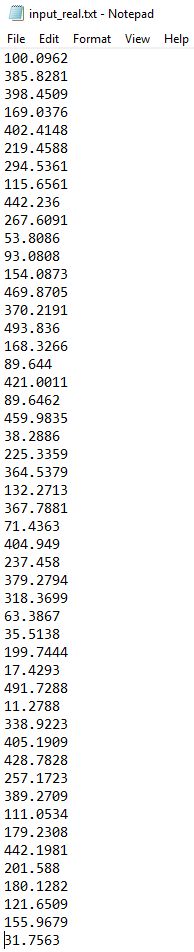
\includegraphics[width=\textwidth]{Input_floatingReal}
\caption{Real Floating Numbers As Input}
\label{Fig_InputfloatingReal} 
\end{minipage}
\end{figure}

\begin{figure}[h!]
\centering
\begin{minipage}[b]{0.5\textwidth}
 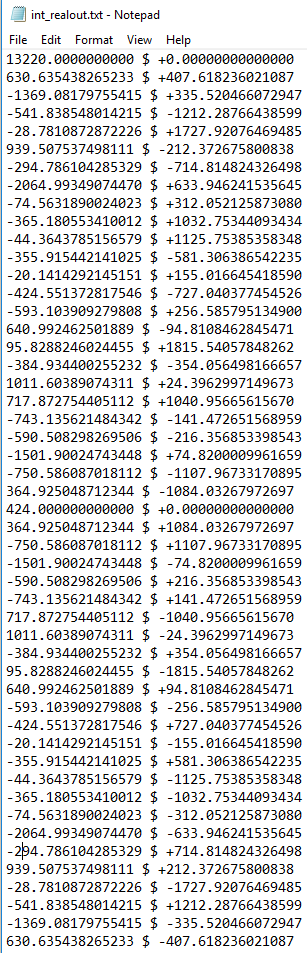
\includegraphics[width=\textwidth]{Output_Real}
\caption{Output For Integer Real Numbers As Input}
\label{Fig_OutputReal} 
\end{minipage}
\hfill
\begin{minipage}[b]{0.32\textwidth}
 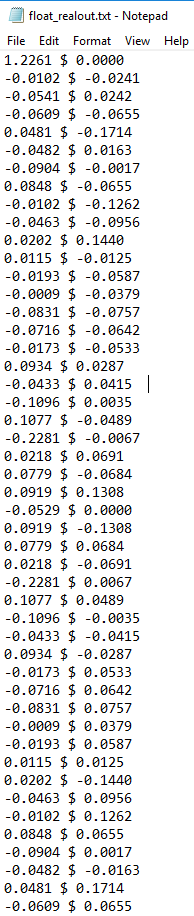
\includegraphics[width=\textwidth]{Output_floatingReal}
\caption{Output For Floating Real Numbers As Input}
\label{Fig_OutputfloatingReal} 
\end{minipage}
\end{figure}
					
\paragraph{Radix-2 Real Number Calculation Function\\}

\begin{enumerate}

\item{\textbf{T-\refstepcounter{tnum}\thetnum \label{R2RFFT}:Radix-2 Real Number FFT Calculation Function}}

\textbf {Type}: Functional, Dynamic, Automated
					
\textbf {Initial State}: None
					
\textbf {Input}:\\{\large input.txt} :  Includes all the input datas. Two examples of input.txt is shown in Figure~\ref{Fig_Inputreal} and Figure~\ref{Fig_InputfloatingReal}. The floating numbers and he integer numbers can be generated by on line random number generators.\\\\
{\large expectedOutput.txt}:  Includes the output datas using the same input datas but computed by Matlab FFT library. Then expectedOutput.txts  are shown in Figure~\ref{Fig_OutputReal} and Figure~\ref{Fig_OutputfloatingReal}. \\ 
If the numbers of data can not satisfy $2^n$, program will automatically fill with 0.\\
					
\textbf {Output}: \\{\large output.txt} : Includes the output datas using the input data computed by this FFT library.\\
{\large TestResult}: pass or not pass. Whether the program passed the test is measured by an admissible error and the algorithm is same as it in T-1.\\
					
\textbf {How test will be performed}: \\
Same as above.

\item{\textbf{T-\refstepcounter{tnum}\thetnum \label{R2RIFFT}:Radix-2 Real Number IFFT Calculation Function}}

\textbf {Type}: Functional, Dynamic, Automated
					
\textbf {Initial State}: None
										
\textbf {Input}:\\{\large input.txt} :  Includes all the input datas. The datas of  input testing file can use the same datas from output.txt from T-3 showed  in Figure~\ref{Fig_OutputReal} and Figure~\ref{Fig_OutputfloatingReal}.\\\\
{\large expectedOutput.txt}:  Includes the output datas using the same input datas but computed by Matlab IFFT library. \\ 
If the numbers of data can not satisfy $2^n$, program will automatically fill with 0.\\
					
\textbf {Output}: \\{\large output.txt} : Includes the output datas using the input data computed by this IFFT library.\\
{\large TestResult}: pass or not pass. Whether the program passed the test is measured by an admissible error and the algorithm is same as it in T-1.\\
					

\textbf {How test will be performed}: \\
Same as above.
\end{enumerate}

\paragraph{Radix-3 Complex Number Calculation Function\\}

\begin{enumerate}

\item{\textbf{T-\refstepcounter{tnum}\thetnum \label{R3CFFT}:Radix-3 Complex  Number FFT Calculation Function}}

\textbf {Type}: Functional, Dynamic, Automated

\textbf {Initial State}: None
					
\textbf {Input}:\\
{\large input.txt}: Same as input.txt in T-1. Reference   Figure~\ref{Fig_Inputcomplex} and Figure~\ref{Fig_Inputfloating}.\\
{\large expectedOutput.txt}: Same as  expectedOutput.txt in T-1.  Reference Figure~\ref{Fig_OutputComplex} and Figure~\ref{Fig_Outputfloating}.\\
If the numbers of data can not satisfy $3^n$, program will automatically fill with 0.\\
					
\textbf {Output}: \\{\large output.txt} : Includes the output datas using the input data computed by this FFT library.\\
{\large TestResult}: pass or not pass. Whether the program passed the test is measured by an admissible error and the algorithm is same as it in T-1.\\
		
\textbf {How test will be performed}: \\
Same as above.

\item{\textbf{T-\refstepcounter{tnum}\thetnum \label{R3CIFFT}:Radix-3 Complex Number IFFT Calculation Function}}

\textbf {Type}: Functional, Dynamic, Automated
					
\textbf {Initial State}: None
					
\textbf {Input}:\\
{\large input.txt}: Same as input.txt in T-2. Reference Figure~\ref{Fig_OutputComplex} and Figure~\ref{Fig_Outputfloating}.\\
{\large expectedOutput.txt}: Same as  expectedOutput.txt in T-2. \\
If the numbers of data can not satisfy $3^n$, program will automatically fill with 0.\\
					
\textbf {Output}: \\{\large output.txt} : Includes the output datas using the input data computed by this FFT library.\\
{\large TestResult}: pass or not pass. Whether the program passed the test is measured by an admissible error and the algorithm is same as it in T-1.\\

\textbf {How test will be performed}: \\
Same as above.
\end{enumerate}

\paragraph{Radix-3 Real Number Calculation Function\\}

\begin{enumerate}

\item{\textbf{T-\refstepcounter{tnum}\thetnum \label{R3RFFT}:Radix-3 Real Number FFT Calculation Function}}

\textbf {Type}: Functional, Dynamic, Automated
					
\textbf {Initial State}: None
					
\textbf {Input}:\\
{\large input.txt}: Same as input.txt in T-3. Reference  Figure~\ref{Fig_Inputreal} and Figure~\ref{Fig_InputfloatingReal}. \\
{\large expectedOutput.txt}: Same as  expectedOutput.txt in T-3.  Reference  Figure~\ref{Fig_OutputReal} and Figure~\ref{Fig_OutputfloatingReal}.\\
If the numbers of data can not satisfy $3^n$, program will automatically fill with 0.\\
					
\textbf {Output}: \\{\large output.txt} : Includes the output datas using the input data computed by this FFT library.\\
{\large TestResult}: pass or not pass. Whether the program passed the test is measured by an admissible error and the algorithm is same as it in T-1.\\
					
\textbf {How test will be performed}: \\


\item{\textbf{T-\refstepcounter{tnum}\thetnum \label{R3RIFFT}:Radix-3 Real Number IFFT Calculation Function}}

\textbf {Type}: Functional, Dynamic, Automated
					
\textbf {Initial State}: None
					
\textbf {Input}:\\
{\large input.txt}: Same as input.txt in T-4. Reference   Figure~\ref{Fig_OutputReal} and Figure~\ref{Fig_OutputfloatingReal}.\\
{\large expectedOutput.txt}: Same as  expectedOutput.txt in T-4.\\
If the numbers of data can not satisfy $3^n$, program will automatically fill with 0.\\
					
\textbf {Output}: \\{\large output.txt} : Includes the output datas using the input data computed by this FFT library.\\
{\large TestResult}: pass or not pass. Whether the program passed the test is measured by an admissible error and the algorithm is same as it in T-1.\\

\textbf {How test will be performed}: \\
Same as above.


\end{enumerate}
\subsection{Tests for Nonfunctional Requirements}

\subsubsection{Speed Comperation Test}
\begin{enumerate}

\item{\textbf{T-\refstepcounter{tnum}\thetnum \label{R3RIFFT}:Compare Calculation Speed with DFT calculation}}

\textbf {Type}: Dynamic, automated, Manual
					
\textbf {Initial State}: None
					
\textbf {Input}: intput.txt
					
\textbf {Output}: Time
					
\textbf {How test will be performed}: \\
Manually compare the time with the time using DFT Library.

\end{enumerate}

\subsubsection{Loading Library Test}

\begin{enumerate}

\item{\textbf{T-\refstepcounter{tnum}\thetnum \label{Win86}:Under Win X86 plateform}}

\textbf {Type}: Functional, Dynamic, Manual
					
\textbf {Initial State}: None
					
\textbf {Input}: input.txt(can be chosen from any input.txt above mentioned and call the corresponding function.) to an C Language compiler.
					
\textbf {Output}: output.txt
					
\textbf {How test will be performed}: Manual


\item{\textbf{T-\refstepcounter{tnum}\thetnum \label{Mac}:Under Mac OS plateform}}

\textbf {Type}: Functional, Dynamic, Manual
					
\textbf {Initial State}: None
					
\textbf {Input}:  input.txt(can be chosen from any input.txt above mentioned and call the corresponding function.) to an C Language compiler.
					
\textbf {Output}: output.txt
					
\textbf {How test will be performed}: Manual


\item{\textbf{T-\refstepcounter{tnum}\thetnum \label{Compilers}:Different Compilers Under The Same Plateform}}

\textbf {Type}: Functional, Dynamic, Manual
					
\textbf {Initial State}: None
					
\textbf {Input}:  input.txt(can be chosen from any input.txt above mentioned and call the corresponding function.) to different compilers including different versions and different languages.
					
\textbf {Output}: output.txt
					
\textbf {How test will be performed}: Manual


\end{enumerate}


\subsection{Traceability Between Test Cases and Requirements}
Since CA does not include requirements part, the Test Cases will be relevant to IM.\\
T-1, T-2, T-3, T-4 all relevant to IM1 in CA.\\
T-5, T-6, T-7, T-8 all relevant to IM2 in CA.\\			
\section{Unit Testing Plan}
\subsection{Input Check Test}

\begin{enumerate}

\item{\textbf{T-\refstepcounter{tnum}\thetnum \label{CNI}: Check Numbers Of Input Data}}

\textbf {Type}: Functional, Dynamic
					
\textbf {Initial State}: None
					
\textbf {Input}: List of Input Datas
					
\textbf {Output}: Check whether List.length equals $2^n$ or $3^n$ according to Radix
					
\textbf {How test will be performed}: Automated Unit Test


\item{\textbf{T-\refstepcounter{tnum}\thetnum \label{FZ}: Fill Input With 0}}

\textbf {Type}: Functional, Dynamic
					
\textbf {Initial State}: None
					
\textbf {Input}: List of Input Datas 
					
\textbf {Output}: List (The List.length must equal to $2^n$ or $3^n$ according to Radix)
					
\textbf {How test will be performed}:  Automated Unit Test


\item{\textbf{T-\refstepcounter{tnum}\thetnum \label{DTC}: Check whether the input data type is the required data type corresponding to the called Function}}

\textbf {Type}: Functional, Dynamic
					
\textbf {Initial State}: None
					
\textbf {Input}:  List of Input Datas
					
\textbf {Output}: Truee or False (True means the data type is right, False means the data type is wrong.)
					
\textbf {How test will be performed}:  Automated Unit Test


\end{enumerate}		

\subsection{Calculation Test}

\begin{enumerate}

\item{\textbf{T-\refstepcounter{tnum}\thetnum \label{CCC}: Complex Number Calculation Check}}

\textbf {Type}: Functional, Dynamic
					
\textbf {Initial State}: None
					
\textbf {Input}: (1 + 2i)*(2 + 3i)
					
\textbf {Output}: (-5 + 7i)
					
\textbf {How test will be performed}: Automated Unit Test


\item{\textbf{T-\refstepcounter{tnum}\thetnum \label{FZ}: $e^{\frac{-2\pi ki}{N}}$ Calculation Check}}

\textbf {Type}: Functional, Dynamic
					
\textbf {Initial State}: None
					
\textbf {Input}: k = 1, N =4
					
\textbf {Output}: -i
					
\textbf {How test will be performed}:  Automated Unit Test

\end{enumerate}	


\bibliographystyle{plainnat}

\bibliography{SRS}

\newpage

\section{Appendix}

This is where you can place additional information.

\subsection{Symbolic Parameters}

The definition of the test cases will call for SYMBOLIC\_CONSTANTS.
Their values are defined in this section for easy maintenance.

\subsection{Usability Survey Questions?}

This is a section that would be appropriate for some teams.

\end{document}